\chapter{TacOSのメモリ管理}
\label{tacosMalloc}
TacOSはファーストフィットで可変区画方式のメモリ管理を行う.
メモリ管理はメモリマネージャサーバが担当する.
メモリマネージャサーバは,
OSがプロセス領域等を割り付けるために使用するサーバプロセスである.
メモリマネージャサーバのソースコードは,
\url{https://github.com/tctsigemura/TacOS/blob/master/os/mm/mm.cmm}
から入手可能である.
プロセス内部でヒープ領域を管理するプログラム
(\|malloc()|、\|free()|)のアルゴリズムも基本は同じである.

TacOSのサーバプロセスはマイクロカーネルにリンクされ
一つのプログラムモジュールになる(\figref{tacosOrganization}参照).
このプログラムモジュールをカーネルと呼ぶ.
メモリマネージャサーバもカーネルの一部である.

%==============================================================================
\section{データ構造の初期化}
メモリ管理用構造体(\|MemBlk|)の宣言と,
初期化プログラムをリスト\ref{tacosMemBlk}に示す.
変数\|memPool|と番兵(\|MemBlk|構造体)は,
カーネルがメモリにロードされた時点で,
カーネルのデータ領域に初期化された状態で置かれる.
\|_end|はカーネルが使用している領域の最後の
アドレス(空き領域の先頭のアドレス)を知るために用いる特殊な名前である.
\|mmInit()|関数はカーネルが起動する際に一度だけ実行され
データ構造の初期化を行う.
\|mmInit()|関数は,まず,空き領域の先頭部分を \|MemBlk| 構造体と見做し
番兵の\|next|がこの構造体を指すようにする(18行).
次に空き領域サイズを計算し,この構造体の\|size|に代入する(19行).
更に,この構造体がリストの最後になるように
\|next|に\|null|を代入する(20行).

\lstinputlisting[numbers=left,label=tacosMemBlk,float=btp,
  firstline=52,lastline=72,
  caption=データ構造と初期化]{TacOS/mm/mm.cmm}

以上の初期化処理が完了した時点のデータ構造を\figref{mmInit}に示す.
\|memPool|変数を起点に番兵付きで長さが1の空き領域リストが完成している.
カーネルはメモリの\|0000H|番地から配置される.
この領域にカーネルのプログラムとデータがロードされる.
図では分かりにくいが,\|memPool|変数と番兵はこの領域に配置される.
最初は,カーネルの直後からメモリ最後の使用不可領域の直前までが
一つの空き領域になっている.
空き領域の先頭に\|MemBlk|構造体を置いたと見做し,
番兵がそこを指すように初期化する.
空き領域先頭の\|MemBlk|構造体が空き領域サイズを記憶し,
\|E000H|番地まで空き領域が続いていることを表現している.

\begin{myfig}{btp}{初期化直後のデータ構造}{mmInit}
  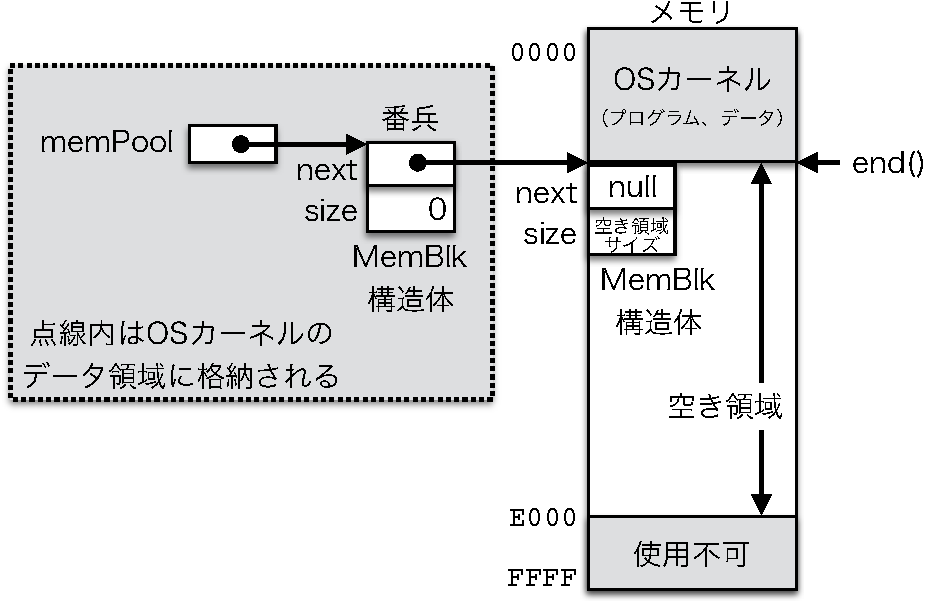
\includegraphics[scale=0.66]{Fig/mmInit-crop.pdf}
\end{myfig}

%==============================================================================
\section{メモリの割り付け}
メモリ領域の割り付けは\|mmAlloc()|関数が行う.
\|mmAlloc()|関数は引数に与えられたバイト数の領域を割り付け,
領域の先頭アドレスを返す.
リスト\ref{alloc}の手順で1KiBの領域を三つ割り付けた状態を
\figref{mmAlloc}に示す.
\|mmAlloc()|は,空き領域の前半に,要求された大きさの領域を割り付ける.
リスト\ref{alloc}では\|mmAlloc()|が3回実行され,
メモリの先頭に1KiBの使用中領域を三つ割り付けている.
その結果,空き領域が小さくなっている.

\begin{lstlisting}[float=btp,label=alloc, caption=1KiBの領域を三つ割り付ける]
  a = mmAlloc( 1024 );      // 1KiB の領域を割り付ける
  b = mmAlloc( 1024 );      // 1KiB の領域を割り付ける
  c = mmAlloc( 1024 );      // 1KiB の領域を割り付ける
\end{lstlisting}

\begin{myfig}{btp}{三つの領域を割り付けた状態}{mmAlloc}
  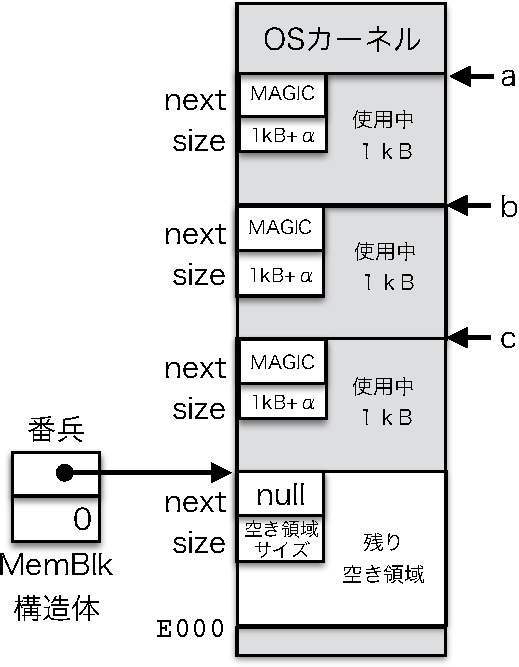
\includegraphics[scale=0.66]{Fig/mmAlloc-crop.pdf}
\end{myfig}

リスト\ref{mmAlloc}に\|mmAlloc()|関数の本体を示す.
\|mmAlloc()|関数は領域の要求サイズ(2行目の\|siz|)を引数に呼び出され,
割り付けた領域のアドレスを整数(\|int|型)で返す.
実際に割り付ける領域は,
要求されたサイズに\|MemBlk|構造体のサイズを加えた後に
偶数に切上げた大きさである(3行目).
TaCでは16bitデータ(2バイトデータ)をメモリに格納する時,
連続した$2i$番地と$2i+1$番地($i$は適当な整数)を使う決まりになっているので,
領域は常に偶数番地から始まるようにする必要がある\footnote{
  割り当てた領域が2バイト(16ビット)データの配列として
  使用される場合を想像して欲しい.}.

\lstinputlisting[numbers=left,float=btp,label=mmAlloc, 
  firstline=77,lastline=102,
  caption=メモリ割り付けプログラム]{TacOS/mm/mm.cmm}

\|mmAlloc()|関数は,
空き領域リストを探索し割り付けるサイズ以上の領域を見つける(7行〜).
サイズ比較に使用される\|_uCmp()|関数は符号なし整数用の大小比較関数である.
領域を探す間はポインタ\|m|が目的の領域を,
ポインタ\|p|が一つ前の領域を指している.
リストの最後に達した場合は,適切な領域が見つからなかったことになる.
\|mmAlloc()|関数は0を返して終了する.

適切な領域(\|m|)が見つかったら,
それを使用領域と空き領域に分割するべきか判断する(13行).
ちょうどピッタリか少しだけ大きい領域なら分割しない.
分割しない場合は領域をリストから外す(16行).

分割する場合は領域の前半(\|m|)を使用領域,残りを空き領域とする.
空き領域のアドレスは,
アドレス用の足算関数\|_addrAdd()|で\|n|に求める(18行).
領域\|m|をリストから外し
代わりに領域\|n|をリストに挿入する(19行〜21行).
領域\|n|の大きさを設定する(22行).

最後に,
領域\|n|が正当に割当てられたことを表すマジックナンバー(\|MAGIC|)を
\|next|に書込む(24行).
\|mmAlloc()|関数が返すアドレスは\|MemBlk|構造体直後である(25行).
\|MAGIC|は\|mmFree()|関数が領域を解放する時に,
正当に割当てられた領域かどうかチェックするために使用される.

%==============================================================================
\section{メモリの解放}
\|mmFree(b);|を実行し領域\|b|を開放した状態を\figref{mmFree1}に示す.
続けて\|mmFree(c);|実行し領域\|c|も開放した状態を\figref{mmFree2}に示す.
\figref{mmFree1}では,領域\|b|が開放され空き領域が二つになり,
空き領域リストの長さが2になっている.
\figref{mmFree2}では,
領域\|c|が開放され空き領域を一つに合体することができたので,
空き領域リストの長さが1になっている.

\begin{figure}[btp]
  \begin{center}
    \begin{minipage}{0.49\columnwidth}
      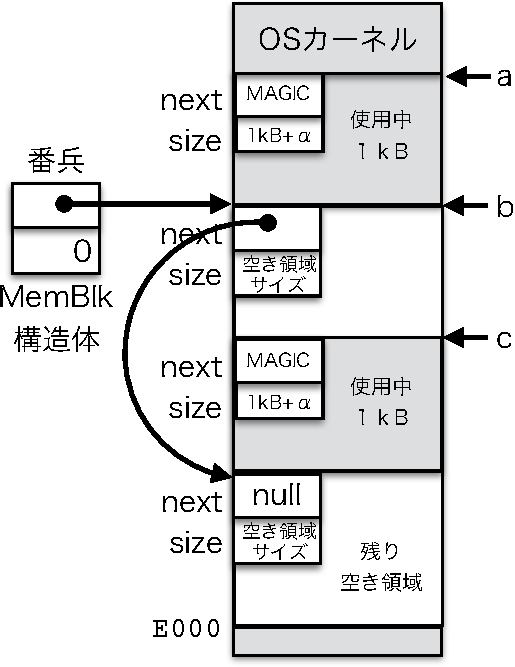
\includegraphics[scale=0.66]{Fig/mmFree1-crop.pdf}
      \caption{領域bを開放した状態}\label{fig:mmFree1}
    \end{minipage}
    \begin{minipage}{0.49\columnwidth}
      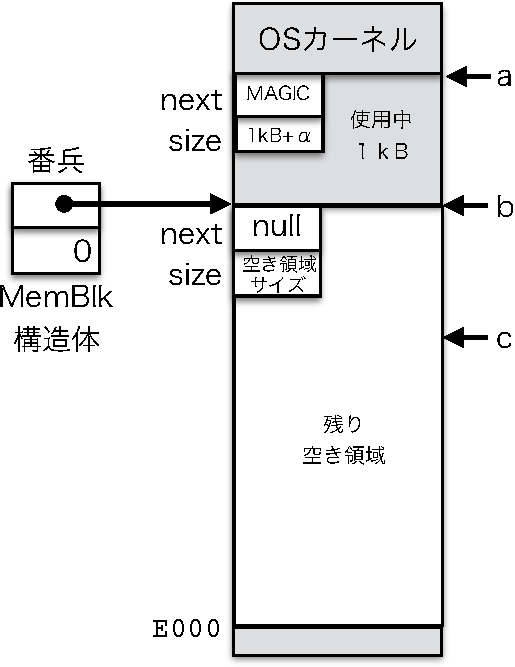
\includegraphics[scale=0.66]{Fig/mmFree2-crop.pdf}
      \caption{領域cも開放した状態}\label{fig:mmFree2}
    \end{minipage}
  \end{center}
\end{figure}

メモリの解放を行う\|mmFree()|関数の本体をリスト\ref{mmFree}に示す.
\|mmFree()|関数は解放する領域\|mem|を引数に実行される(2行).
領域の\|MemBlk|構造体に\|MAGIC|が格納されていない場合は
\|mmAlloc()|関数で割り付けられた正当な領域では無いので
エラーを表示してシステムを停止する(8行)\footnote{
  このプログラムはOS内部で動くものである.
  このような事象が発生するのはOSのバグが原因と考えられるので
  システムを停止する.}.

\lstinputlisting[numbers=left,float=btp,label=mmFree,
  firstline=108,lastline=144,
  caption=メモリ解放プログラム]{TacOS/mm/mm.cmm}

解放された領域は新しい空き領域になる.
空き領域リストがアドレス順になるように,
新しい空き領域を挿入すべき位置を探す処理を行う(10行〜).

解放する領域が直前の空き領域に重なっていたり,
直後の空き領域に重なっていたりしていないかチェックしている(19行)\footnote{
  これもOSのバグ以外では発生しない.
  OS自身がバグを含んでいないかチェックする機会として利用している.}.

解放する領域が直前の空き領域に隣接している場合は,
直前の空き領域サイズを大きくすることで一つの空き領域にする(23行).
直後の空き領域とも隣接している場合は,
直前の空き領域サイズを更に大きくし直後の空き領域も一つの領域にする(25行).
この時は,空き領域が一つにまとめられたので,
空き領域リストから直後の空き領域を削除する(26行).

更に,直後の空き領域だけと隣接している場合(28行),
どの空き領域とも隣接していない場合(32行)の処理が続いている.

%==============================================================================
\section{まとめ}
本章では,TacOSのメモリ管理プログラムを例に,
ファーストフィット方式を用いる可変区画方式の
メモリ割り付けプログラムを紹介した.
